\chapter{Identificación de requerimientos}
\label{cap:reqUsr}

	En este capítulo se modela el alcance del sistema,
	

%---------------------------------------------------------
\section{Objetivo General Del Proyecto}
Llevar  el  control  completo  de  la  farmacia,  mediante  un   único  sistema  conectado  y utilizado por todos los empleados en las diferentes sucursales de la franquicia.
\section{Objetivos Específicos}
\begin{itemize}
\item Resolver los problemas que surjan en el entendimiento del negocio.

\item Reducir los problemas de inventario con base a las salidas  y entradas de medicamento.

\item Tener una visión del general sobre el ámbito laboral de las múltiples sucursales como de los empleados que operan en ella.

\end{itemize}

\section{Requerimientos del Usuario}
\begin{itemize}

\item RU1 Registrar Medicamentos\\
Descripción: El dueño necesita registrar los nuevos medicamentos que se venderán en la farmacia.\\
\item RU2 Registrar entregas de proveedores\\
Descripción: El cajero necesita registrar los medicamentos que llegarón de un proveedor, de la misma forma necesita información del proveedor que hace la entrega ,requiere la hora y fecha en que se realizó la entrega, y un comprobante de parte del proveedor.\\

\item RU3 Consultar Medicamento por cada Sucursal\\
Descripción:El usuario necesita conocer el medicamento que se maneja así como la cantidad de cada uno de estos medicamentos por cada una de las sucursales.\\

\item RU4 Registrar Empleados\\
Descripción:El dueño necesita tener una forma para registrar la información de los nuevo trabajadores que laboran en la franquicia de la farmacia, de la misma manera necesita asignarles sucursal para laborar; en caso de que sea supervisor asignarle un máximo de 3.\\

\item RU5 Control de la caja.
Descripción: El dueño necesita que alguien monitorice el dinero con el que se empieza cada turno (matutino, vespertino, nocturno) así como al final de estos.\\

\item RU6 Realizar una Venta\\
Descripción: El cajero requiere registrar nombre,costo y unidades de cada medicamento en la venta.\\

\item RU7 Registrar Sucursal\\
Descripción: El dueño requiere registrar información de cada nueva sucursal( dirección,el nombre y teléfono).\\

\item RU8 Consultar Ventas por día\\
Descripción: El supervisor necesita conocer las ventas que se realizaron durante la hora de atención de la farmacia(9:00am A 12:00pm) para tener una visión de las ventas.\\

\item RU9 Registrar Proveedor
Descripción: El dueño Necesita Registrar a los proveedores que le surten de medicamentos.\\

\item RU10 Consultar Proveedores
Descripción: El dueño necesita consultar a los proveedores para hacer algún pedido,
o en su defecto aclarar algún inconveniente.\\

\item RU11 Recibir Medicamentos\\
Descripción: El cajero necesita modificar las existencias de los medicamentos que se venderán en la farmacia conforme a entregas de los proveedores.\\
\end{itemize}
\newpage
\section{Requerimientos funcionales}
RF1 Registrar Medicamento\\
Descripcion: El sistema Guarda la información de forma estructurada de los campos de importancia de un medicamento, como su nombre, ingredientes Activos con su dosificación, Precios de compra y venta, caducidad, presentación, vía de administración, laboratorio,lote,advertencias y existencias\\
Prioridad: MA\\
RU:RU1.\\
\\
RF2 Registrar Entregas 
Descripcion: El sistema guarda la información de las entregas realizadas por el proveedor tales como fecha, hora, proveedor, y todos los campos mencionados en la entidad ``Ingreso" y también en la entidad ``Lote" En la Sección ``Modelo del dominio del problema" en el  Capitulo anterior.\\
Prioridad:A\\
RU:RU2.\\
\\
RF3 Registrar Clientes\\
Descripcion:El Sistema Guarda información de un cliente, los campos que Guarda del Cliente están Especificados en la entidad ``Cliente" En la Sección ``Modelo del dominio del problema" en el  Capitulo anterior.\\
Prioridad:M\\
RU:RU3\\
\\
RF4 Registrar Empleados\\
Descripcion: El sistema guarda la información de un empleado, este Empleado puede ser un Cajero o un Supervisor, la información que guarda de cada uno de estos empleados esta Especificada en las Entidades ``Cajero" y ``Supervisor" En la Sección ``Modelo del dominio del problema" en el  Capitulo anterior.\\
Prioridad:A\\
RU:RU4\\
\\
RF5 Abrir Caja\\
Descripcion:El sistema Permite Que el usuario pueda Abrir la Caja y Muestra el dinero con el que se Cerro la caja en el turno anterior para mostrarlo al usuario.\\
\\
Prioridad:A\\
RU:RU5
\\
RF6 Cerrar caja\\
Descripcion: El sistema Permite Que el usuario Pueda cerrar la Caja, y Calcula El dinero de las ventas realizadas a lo largo del turno, lo muestra en pantalla para el usuario y lo guarda como una variable temporal(hasta Que se abre turno)\\
Prioridad:A\\
RU:RU5\\
\\
RF7\\
Nombre: Realizar Una Venta\\
Descripcion:El sistema cuando se realiza una venta Guarda todos los datos especificados en la entidad ``Venta" y la entidad ``detalle Venta" En la Sección ``Modelo del dominio del problema" en el  Capitulo anterior, Aparte en el mismo proceso reduce las existencias del medicamento que se vendió e imprime un comprobante con la información de ``Venta" desde una impresora\\
Prioridad:MA\\
RU:RU6\\
\\
RF8 Consultar Medicamento Local\\
Descripcion: El sistema Mostrara una tabla con los medicamentos que se tienen en la sucursal y datos esenciales como su nombre, precio, Existencias y proporciona al usuario un botón para que pueda visualizar toda la información del medicamento.\\
Prioridad:M\\
RU:RU7\\
\\
RF9 Registrar Sucursal\\
Descripcion: El sistema Guarda la información de una sucursal la cual se especifica en la entidad ``Sucursal" En la Sección ``Modelo del dominio del problema" en el  Capitulo anterior. \
Prioridad:A\\\
RU:RU8\\
\\
RF 9 Consultar Ventas Por día\\
Descripcion: El sistema un reporte en formato .pdf donde se desglosan las ventas del día, Los datos que se desglosan en el reporte son el nombre del medicamento y el precio del mismo.\\
Prioridad: MA\\
RU:RU9\\
\\
RF13 Registrar Proveedor
Descripcion: El sistema guardara la Información de el proveedor La Cual se especifica en la entidad ``Proveedor" En la Sección ``Modelo del dominio del problema" en el  Capitulo anterior.\\
Prioridad: A\\
RU:RU10\\
\\
RF14 Consultar Proveedor\\
Descripcion: El sistema muestra una tabla que en lista a los proveedores que estan registrados en el sistema junto con sus datos especificados En la Sección ``Modelo del dominio del problema" en el  Capitulo anterior.
Prioridad: M\\
RU:RU11\\
\newpage

%---------------------------------------------------------
\section{Especificación de plataforma}	

\begin{description}

	\item[Tipo de sistema:] Web.
	\item[Software requerido:]Apache, Maria-DB,google-chrome,firefox,edge.
	\item[OS:] Arch Linux x86\_64.
	\item[Kernel Release:] 4.14.47-1-MANJARO.
	\item[RAM:] 2006 MB / 3835 MB
	\item[Processor Type:] Intel(R) Celeron(R) CPU B830 @ 1.80GHz.
	\item[servicios:] servicios del servidor de base de datos 10.1.33-MariaDB MariaDB Server.\\También se Ocupan servicios del serve API Apache 2.0 Handler
Con la Version de Apache:	Apache/2.4.33 (Unix) PHP/7.2.6.
	\item[Mysql Support:] mysqlnd 5.0.12-dev - 20150407.
	\item[Hosting:]Se Compra un servidor dedicado con el proveedor ``Go Daddy".
	Se compra un servidor dedicado, para que se pueda dar soporte a  todos los empleados en todas las sucursales,tal vez al principio se tendrá espacio y servidor de sobra, pero de esta forma aumenta la productividad y se quitan los riesgos de trafico en el servidor.
	\item[servidor Hosting:]4 núcleos de CPU @ 3.1 GHz
Memoria de 4 GB
1 TB de almacenamiento (RAID-1)\^
Ancho de banda sin medición(El proveedor no limita el ancho de banda) 
3 IP dedicadas
Certificado SSL gratis durante 1 año.
	\item[Dominio:] Se Compra el dominio ``www.Farmacias.francs.com"\\  con el mismo proveedor a un precio muy razonable con contrato de un año al igual que el servicio de hosting.
	\item[Seguridad web:]El mismo proveedor de hosting ofrece seguridad SSL
	con las siguientes Caracteristicas:Asegura un sitio web
Sólido cifrado SHA2 y encriptación de 2048 bits\\
Disponible en Certificados SSL DV, OV y EV.\\
El SSL EV hace que la barra del navegador se ponga verde 
Incrementa el posicionamiento de tu sitio en Google.\\
Marca confiable McAfee SECURE.\\
\end{description}
\begin{figure}[htbp!]
	\begin{center}
		\fbox{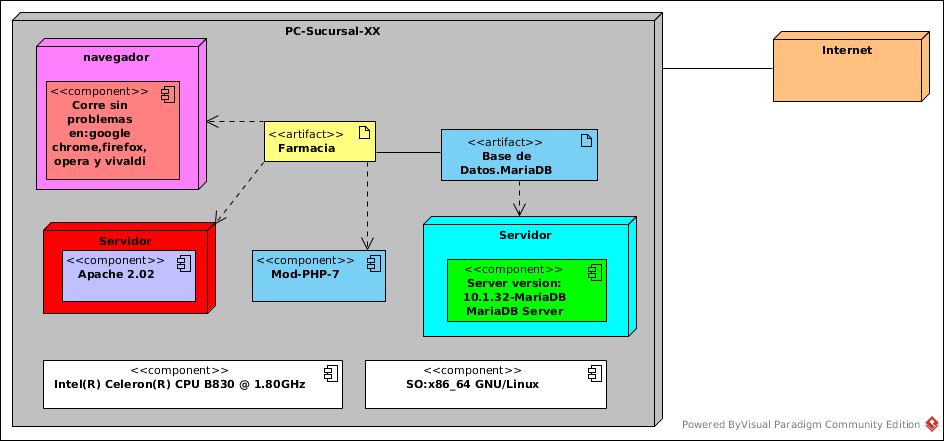
\includegraphics[width=18cm, height=20cm]{images/arquitectura}}
		\caption{Arquitectura del sistema.}
		\label{fig:arquitectura}
	\end{center}
\end{figure}

En la figura~\ref{fig:arquitectura} se describe la estructura del sistema, en ella se detalla los servicios de base de datos que se necesitan, las conexiones al servidor apache, así como las especificaciones que necesita el CPU de la sucursal en la que se monta el sistema de la farmacia.



